\documentclass[letterpaper]{article}
\usepackage[utf8]{inputenc}
\usepackage[parfill]{parskip}    % Activate to begin paragraphs with an empty line rather than an indent
\usepackage{graphicx}
\usepackage{amssymb}
\usepackage{amsmath}
\usepackage{amsthm}

\usepackage{afterpage}

\usepackage{algorithm}
\usepackage{algpseudocode}

\usepackage{verse}

\newtheorem{theorem}{Theorem}[section]
\newtheorem{corollary}{Corollary}[theorem]
\newtheorem{lemma}[theorem]{Lemma}

\theoremstyle{remark}
\newtheorem*{remark}{Remark}

\usepackage{epstopdf}
\usepackage{circuitikz}
\usepackage[separate-uncertainty = true,multi-part-units=single]{siunitx}
\usepackage{booktabs}
\usepackage{enumitem}
\usepackage[toc,page]{appendix}
\usepackage{color}
\usepackage{pgfplots}
\usepackage{pgfplotstable}
\usepackage{caption}
\usepackage{subcaption}
\usepackage{url}
\usepackage{multirow}
\usepackage{makecell}
\usepackage[round]{natbib}   % omit 'round' option if you prefer square brackets
\usepackage{titling}
\usepackage{siunitx}

\usepackage{setspace}
% \doublespacing
\usepackage{float}

\pgfplotsset{compat=1.14}


\usepackage{fancyhdr}

\pgfplotscreateplotcyclelist{grayscale}{
    thick,white!10!black,mark=x,mark options=solid, dashed\\%
    thick,white!20!black,mark=o,mark options=solid\\%
}


\newcommand{\answer}[1]{\framebox{$\displaystyle #1 $}}

 
\pagestyle{fancy}
\fancyhf{}
\rhead{David Shi}
\lhead{CS61C}
\cfoot{\thepage}

\title{Lecture 1 - Notes}
\author{David Shi}
\date{June 2019}
\begin{document}

\maketitle

\section{Overview}

In this introductory lecture, we were given introductions to our professors, TAs, and tutors. We also covered a high level overview of the class in terms of the course's goals and objectives. We discussed the importance of the course policies before diving in to our first topic on number representation.

\section{Course Overview}

We first discussed the two major goals of the course, those being to answer the two questions:
\begin{itemize}
  \item How do computer processors and memories work, and how do they affect software design and performance?
  \item Introduction to “computer systems” areas: architecture, compilers, security, embedded, operating systems, large-scale computing
\end{itemize}
The ways in which hardware and software interacted was abstracted into a figure such as the the one provided:

\begin{figure}[t]
    \caption{How hardware and software concepts stack}
    \label{fig:my_label}
\end{figure}
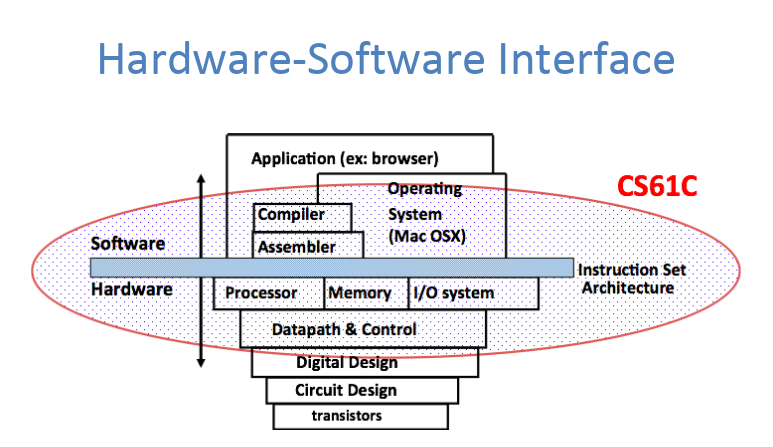
\includegraphics[scale=.5]{Capture}

The red circle indicates the material that this course covers, emphasized on the interactions between software and hardware.
\subsection{Computer Architecture of Software Development}

Many of the students who take this course likely care more about the software side of computer science \textit{(myself included)}. However, there are many reasons that understanding the computer architecture is still important for software developers. These reasons include understanding the machine that we are using to do our work. We can also understand how performance matters, and take advantage of certain principles such as parallelism when developing software. There are also certain ways that different programming languages behave through the computer. However, the last and likely more \textbf{important} reason computer architecture is important for software engineers is understanding design methodology and thinking of designs in terms of limitations and trade-offs.

\subsection{Course Learning Objectives}

One of the most important things to understand when going in to a new class is likely knowing what the objectives of the class are, and knowing what we are expected to know after completion of the course. We summarized these course objectives in to the following list of things we should be able to do:
\begin{itemize}
    \item Identify and explain the various layers of abstraction that allow computer users to perform complex software tasks without understanding what the computer hardware is actually doing
    \item Judge the effect of changing computer components (e.g.processor, RAM, HDD, cache) on the performance of a computer
    \item Explain how the memory hierarchy creates the illusion of being almost as fast as the fastest type of memory and almost as large as the biggest memory program
    \item Construct a working CPU from logic gates for a specified instruction set architecture
    \item Identify the different types of parallelism and predict their effects on different types of applications
\end{itemize}
In addition, we were given a list of skills we as students should be developing and considering throughout this course:
\begin{itemize}
    \item Creating and modifying designs to meet a given set of specifications
    \item Identifying unexpected or problematic situations using debugging tools, and creating test cases to ensure proper behavior
    \item Defending design choices based on trade-offs and limitations
\end{itemize}

\subsection{The 6 Great Ideas in Computer Architecture}

The 6 Great Ideas in Computer Architecture are the most important concepts involved in Computer Architecture. We can also view these 6 ideas as the 6 sections that are covered throughout the class. Our 6 ideas are the following items:
\begin{itemize}
    \item Abstraction
    \item Technology Trends
    \item Principle of Locality/Memory Hierarchy
    \item Parallelism
    \item Performance Measurement and Improvement
    \item Dependability via Redundancy
\end{itemize}
We begin the course with the first great idea: \textbf{Abstraction}

\section{Course Policies}
All of this information being available on the website: 
https://cs61c.org/policies/, 
Make sure that you understand these course policies very well to avoid any logistical issues that can potentially harm your grade.

\section{Number Representation}
We have been accustomed to thinking of numbers in terms of base tens since we count on our fingers. The other common bases we will be working with are \textbf{binary} (base 2) and \textbf{hexadecimal} (base 16). \textbf{Decimal numbers} have symbols ranging from 0 to 9. \textbf{Binary numbers} have the symbols 0 and 1. \textbf{Hexadecimal numbers} have symbols from 0 to 9, as well as the letters a-f to represent 10-15.

The \textbf{Big Idea} that we were told to remember from this lecture was the idea that bits can be used to represent absolutely anything, entirely depending on our interpretation. This means if we choose to interpret bits to represent characters, that is allowed.

\section{Assignment Schemes}
When we design schemes for what our bits should be assigned to, there are several criteria we should use to evaluate how effective of a design it is. The criteria are as follows:
\begin{itemize}
    \item \textbf{Zero:} we would prefer if the Zero of our design has 0...0 representing 0
    \item \textbf{Most Negative Number:} We need our design to encapsulate any possible numbers for our design, so we want to reach as many negative numbers as we need
    \item \textbf{Most Positive Number:} likewise to the most negative number, we need to be able to access as many positive numbers as we need
    \item \textbf{Increment:} Possibly the most important criteria, we need our system for adding values together to make sense in terms of the bits. Most ideal increment would be adding the bits of one value to the bits of another value would equal the correct value always.
\end{itemize}

Let us consider several assignment schemes in terms of these criteria and consider the pros and cons of each system.

\subsection{Unsigned Integers}
This system only contains positive integers, with no negative integers at all. This system is effective if we only need to consider positive integers. In terms of our 4 criteria:
\begin{itemize}
    \item \textbf{Zero:} our zero value is contained in 0...0, so this criteria checks off
    \item \textbf{Most Negative Number:} zero is our most negative value since we don't have negative values. This does not matter if we don't need to consider negative numbers
    \item \textbf{Most Positive Number:} our most positive number is $(2^n - 1)$
    \item \textbf{Increment:} Increments correctly
\end{itemize}
In summary, the pros of using Unsigned Integers are that the zero is correct, increments make sense, and the numbers are easy for us to translate. The only real con is that we can't utilize negative numbers with unsigned integers. Next, we will evaluate some methods that allow us to utilize negative integers as well as positive integers.

\subsection{Sign and Magnitude}
The first logical system we might think of to include negative numbers is to make the Most Significant Bit (the leftmost bit) a 1 if our number is negative and 0 if our number is positive. This would define our system of \textbf{Sign and Magnitude}. Let us evaluate our system with our criteria:
\begin{itemize}
    \item \textbf{Zero:} We unfortunately have 2 different values for 0, one positive and one negative, which mathematically doesn't make sense.
    \item \textbf{Most Negative Number:} $-(2^(n-1) - 1)$
    \item \textbf{Most Positive Number:} $2^(n-1) - 1$
    \item \textbf{Increment:} Our incrementing system does not work correctly.
\end{itemize}
Overall, this system is very easy to think of, but does not work very well since we have 2 zeros and incrementing does not make sense with this system. Let us consider another system.

\subsection{Biased Notation}
In this system, we take the unsigned integer system and "shift" the values so that 0 is roughly in the middle. (Value = "unsigned value" - bias), with bias typically being $(2^{n-1} - 1)$. Let us evaluate this system with our criteria:
\begin{itemize}
    \item \textbf{Zero:} The zero becomes the Bias, which is suboptimal for a system
    \item \textbf{Most Negative Number:} Our most negative number becomes our bias
    \item \textbf{Most Positive Number:} Our most positive number becomes the bias+1
    \item \textbf{Increment:} Works similarly to unsigned. 
\end{itemize}
Overall, the system is quite easy to increment, but the main con is that the zero doesn't match 0 and therefore is not a logical value for zero. Let us consider a system that uses bit complementing.

\subsection{One's Complement}
In this system, we find the negative value of an integer by complementing the bits, or changing 1's to 0's and 0's to 1's. For example: 0b001 evaluates to 1, and 0b110 evaluates to -1. We can also observe that the Most Significant Bit (the leftmost bit), is a 1 for negative numbers and 0 for positive numbers. Let us evaluate this system:
\begin{itemize}
    \item \textbf{Zero:} We unfortunately have 2 values for 0, 0b0...0 and 0b1...1. Suboptimal
    \item \textbf{Most Negative Number:} Our most negative number is $-(2^{n-1} - 1)$
    \item \textbf{Most Positive Number:} Our most positive number is $(2^{n-1} - 1)$
    \item \textbf{Increment:} Works correctly.
\end{itemize}
This system is so close to being perfect again. It increments perfectly, even between numbers of the opposite signs. The only drawback is that  there are 2 values for 0. Let us tweak this system one more time to find our desired signed integer representation.

\subsection{Two's Complement}
This system works the same as One's Complement, but after taking the complement of an integer to get its negative value, you add decimal value 1 to it. For example: Decimal 1 = 001, and its complement is 110. Adding 1 to 110 gives 111, which is our value for decimal -1. Let us observe why this system is perfect for signed integers:
\begin{itemize}
    \item \textbf{Zero:} We have 1 zero value at 0b00...0
    \item \textbf{Most Negative Number:} Our most negative number is $-(2^{n-1})$
    \item \textbf{Most Positive Number:} Our most positive number is $(2^{n-1} - 1)$
    \item \textbf{Increment:} Works correctly.
\end{itemize}
We can see that this system matches all of our required criteria. One thing to note is that this is the only signed integer system that has one more negative value than positive, rather than having more positive than negative values. This system is used by all modern hardware for signed integers, and we can still look at the Most Significant Bit as a sign bit. It was mentioned in discussion that the main systems we as students should understand well are Two's Complement, Biased Notation, and Unsigned Integers.

\section{Overflow}
Thinking outside the scope of computers, we as math students know that there are an infinite number of digits. This causes problems for us computer scientists as the nature of hardware means we can only have a fixed number of digits.

This brings us to the idea of bit \textbf{Overflow}. Overflow is the result of an arithmetic operation that causes us to not have enough bits to store the new value. In layman's terms, this is when the number we should represent is larger than the number of bits allows us to represent. For example: if we are working with 4 bits and we add the numbers 0b1000 (decimal 8) and 0b1000 (decimal 8), are value mathematically should return decimal 16, but we don't have enough bits to represent 16.

There are 3 main solutions to dealing with overflow. The most simplistic answer is to ignore overflow entirely, which is probably not the best solution to work with when actually in the field of software development. The next potential solution is to throw an error or exception whenever overflow occurs. Similarly to how our calculators show overflow errors when we deal with numbers too large for it to represent. The third, and potentially trickiest solution is to add more bits with an operation known as \textbf{Sign Extension}.

\subsection{Sign Extension:}
Sign Extension is the process of representing the same number with more bits than previously available. A very basic example would be for unsigned integer 0b0001 becoming 0b0000 0001.

Sign Extension is very easy to do for unsigned integers, as we only need to add leading 0's to the original number. For signed integers, sign extension can be potentially tricky to do. 

For \textbf{Sign Magnitude representations}, we need to add 0's after the sign bit. Ex. 0b11 becomes 0b1001.

For \textbf{One's Complement} and \textbf{Two's Complement}, we need to copy the Most Significant Bit. For example: 0b0001 becomes 0b0000 0001 and 0b1001 becomes 0b11111001.

\end{document}